\documentclass{cubeamer}

\usepackage[french]{babel}
\usepackage[T1]{fontenc}
\usepackage{multicol}
\usepackage{hyperref}
\usepackage{url}
\usepackage{xcolor}
% Code enlightement
\usepackage{code-package}

\title{Clustering avec Docker Swarm}
\subtitle{Administration et protocoles réseaux}
\author[Sami Babigeon \& Louka Boivin]{Sami Babigeon \& Louka Boivin}
\date{\today}
\institute[Université de Rouen]{Master 2 SSI}

% Turn off slides numbering with allowframebreaks
\setbeamertemplate{frametitle continuation}{}
% Right arrow
\newcommand{\arrow}{$\rightarrow$ }

\begin{document}

% Title and ToC

\maketitle
\cutoc

% Main section
\section{Docker}

\begin{frame}{Présentation}
    \begin{multicols}{2}
    Docker est une plateforme open-source permettant de concevoir, tester et déployer rapidement
    des applications.
    
    Il utilise la notion de conteneurs qui, comme la virtualisation,
    permet d'isoler une application du serveur hôte tout en étant plus léger et plus simple à
    déployer.

    \columnbreak
    \begin{figure}
        \centering
        
\includegraphics[width=6cm]{img/docker}
    \end{figure}    

    \end{multicols}
\end{frame}

\begin{frame}{Fonctionnement}
    \begin{multicols}{2}
    Docker étend les conteneurs LXC qui s'appuient sur les fonctionnalités du noyau pour
    l'isolation (namespaces, cgroups), en fournissant une API haut niveau, plus simple
    d'utilisation.

    Le Docker Hub est une bibliothèque d'images publics pour créer facilement tous
    types de conteneurs.
    
    \columnbreak
    \begin{figure}
        \centering
        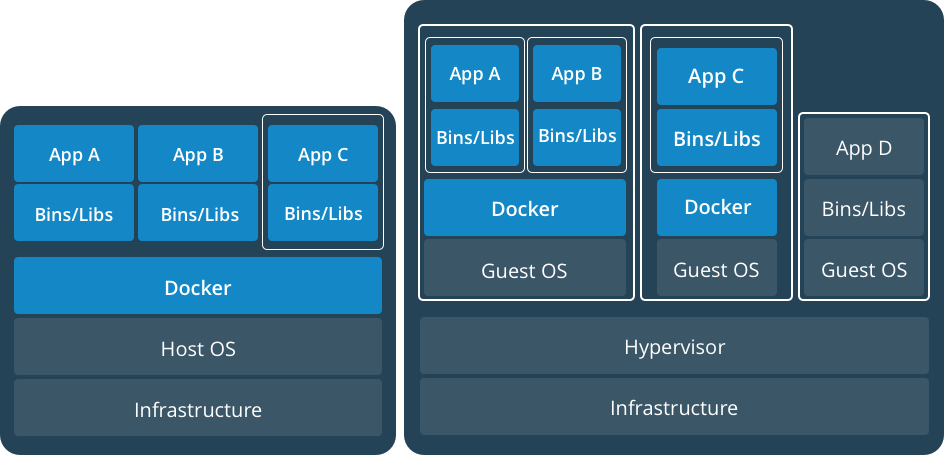
\includegraphics[width=7cm]{img/vm-container}
    \end{figure}    

    \end{multicols}
\end{frame}

\begin{frame}[fragile]{Installation}
    \begin{multicols}{2}
Sur une machine Ubuntu :
\begin{bashResized}{0.48}
sudo apt install docker
sudo systemctl start docker
\end{bashResized}
    \columnbreak
    
Sur MacOS / Windows :
\begin{bashResized}{0.48}
Installer Docker Desktop :
https://www.docker.com/
\end{bashResized}
    \end{multicols}

    Pour pouvoir lancer des commandes docker sans privilèges :
\begin{bash}
sudo usermod -aG docker <username>
\end{bash}
\end{frame}

\begin{frame}[fragile]{Utilisation}
    Puis ensuite pour tester :
\begin{bash}
docker pull python
docker run -it python
\end{bash}

    \begin{figure}
        \centering
        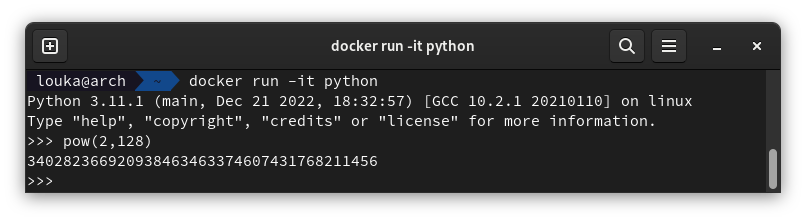
\includegraphics[width=\textwidth]{img/docker-test.png}
    \end{figure}
\end{frame}

\section{Docker Swarm}

% Multicol frame
\begin{frame}{Présentation}
    \begin{multicols}{2}
    Docker Swarm est un outil d'orchestration permettant de créer et gérer des clusters de
    machines physiques ou virtuelles hébergeant une application. C'est un outil intégré à Docker.

    L'interêt principal d'un cluster Swarm est la haute disponibilité que cela procure pour
    l'application.

    \columnbreak
    \begin{figure}
        \centering
        
\includegraphics[width=4cm]{img/swarm}
    \end{figure}

    \end{multicols}
\end{frame}

\begin{frame}{Terminologie}
    \begin{multicols}{2}
        \begin{itemize}
            \item Éléments d'un cluster \arrow \emph{Noeuds (nodes)}
            \item Cluster \arrow \emph{Manager(s) + Workers}
            \item Workers \arrow \emph{Exécution}
            \item Managers \arrow \emph{Orchestration}
        \end{itemize}
    \columnbreak
        \begin{figure}
            \centering
            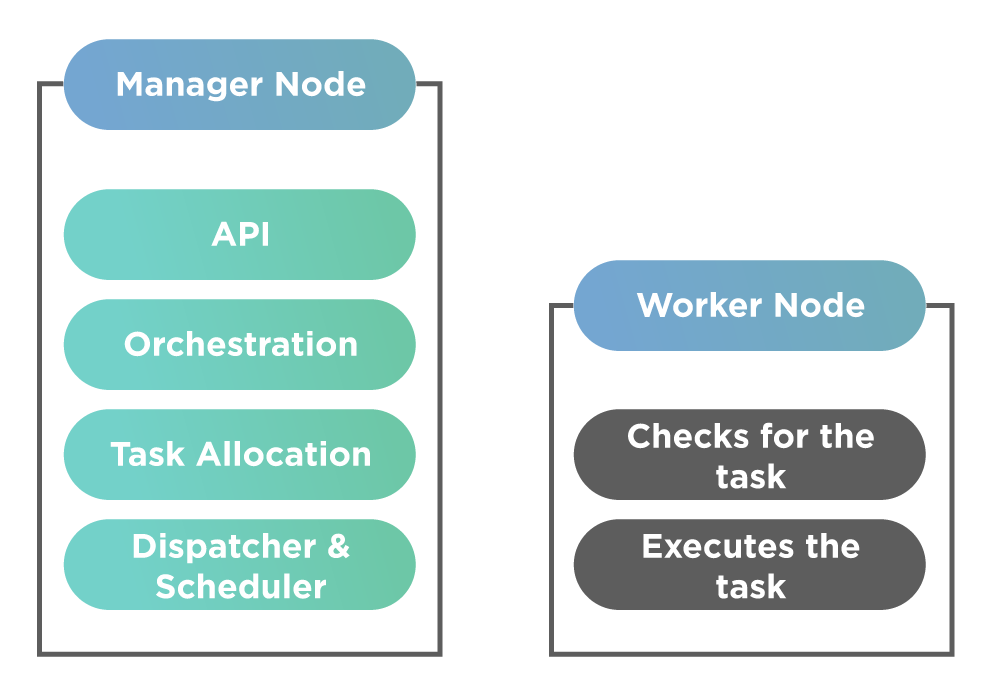
\includegraphics[width=0.5\textwidth]{img/manager}
        \end{figure}
    \end{multicols}
\end{frame}

\begin{frame}{Schéma d'un cluster}
    \begin{figure}
        \centering
        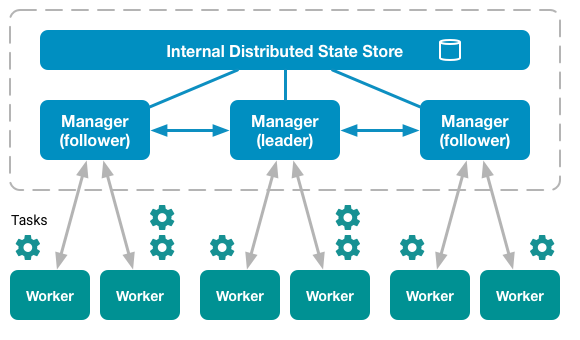
\includegraphics[width=0.85\textwidth]{img/swarm-network}
    \end{figure}
\end{frame}

\begin{frame}{Pourquoi utiliser Swarm ?}
    \begin{multicols}{2}
        \begin{itemize}
            \item Scalabilité
            \item Équilibrage de charges automatique
            \item Retour à l'état souhaité
            \item Mise en réseau multi-hôtes
            \item Sécurité
        \end{itemize}
    \columnbreak
        \begin{figure}
            \centering
            
\includegraphics[width=0.24\textwidth]{img/scalability}
            
\includegraphics[width=0.24\textwidth]{img/load-balancing}
        \end{figure}
    \end{multicols}
\end{frame}

\section{Démonstration}

\section{Conclusion}

% Q&A
\begin{frame}[standout]
    \Huge\textsc{Merci de votre écoute}
    \vfill
    \LARGE\textsc{Questions ?}
\end{frame}

\section*{Bibliographie}

\begin{frame}[allowframebreaks]
    \frametitle{Références}
    \nocite{*}
    \bibliographystyle{acm}
    \bibliography{bibliography}
\end{frame}

\end{document}

